\documentclass[fleqn, a4paper, 12pt]{amsart}
\usepackage{amsmath, amssymb, amsthm}
\usepackage[top=1in, left=1in, right=1in, bottom=1in]{geometry}
\usepackage{gensymb}
\usepackage{commath}
\usepackage{xcolor}
\usepackage{todonotes}
\usepackage{cancel}
\usepackage{siunitx}
\usepackage{tikz, pgfplots}
	\usetikzlibrary{calc, hobby, patterns, intersections}
\usepackage{graphicx}
\usepackage{hyperref}
\usepackage{datetime}
\usepackage{ulem}
\usepackage{xfrac}
\usepackage{asymptote}
\usepackage{enumerate}
\usepackage{float}
\setcounter{secnumdepth}{4}
\newcommand\numberthis{\addtocounter{equation}{1}\tag{\theequation}}

\newcommand{\AxisRotator}[1][rotate=0]{%
	\tikz [x=0.25cm,y=0.60cm,line width=.2ex,-stealth,#1] \draw (0,0) arc (-150:150:1 and 1);%
}

\theoremstyle{definition}
\newtheorem{example}{Example}
\newtheorem{definition}{Definition}

\theoremstyle{theorem}
\newtheorem{theorem}{Theorem}

\newenvironment{solution}
{\begin{proof}[Solution]\let\qed\relax}
	{\end{proof}}

\newcommand{\curl}{\mathrm{curl\,}}

%section headings on left
\makeatletter
\def\specialsection{\@startsection{section}{1}%
	\z@{\linespacing\@plus\linespacing}{.5\linespacing}%
	%  {\normalfont\centering}}% DELETED
	{\normalfont}}% NEW
\def\section{\@startsection{section}{1}%
	\z@{.7\linespacing\@plus\linespacing}{.5\linespacing}%
	%  {\normalfont\scshape\centering}}% DELETED
	{\normalfont\scshape}}% NEW
\makeatother

%forces newline after subsection
\makeatletter
\def\subsection{\@startsection{subsection}{3}%
	\z@{.5\linespacing\@plus.7\linespacing}{.1\linespacing}%
	{\normalfont\itshape}}
\makeatother

%opening
\title{Physics 1 : Assignment 12}
\author{Aakash Jog}
\date{\formatdate{21}{1}{2015}}

\begin{document}

\maketitle
%\setlength{\mathindent}{0pt}

%\tableofcontents

%\newpage
\section*{Week 4 : Class Exercises}

\subsection*{Exercise 1}

\begin{figure}[H]
	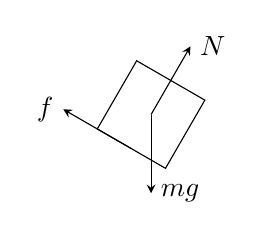
\begin{tikzpicture}
		\def\l{1};
		\def\b{1};
		\def\angle{30};
		\def\F{1};
	
		\begin{scope} [rotate around = {{-\angle}:({\l/2},{\b/2})}]
			\draw (0,0) rectangle (\l,\b);
			
			\coordinate (centre) at ({\l/2},{\b/2});
			\coordinate (base) at ({\l/2},0);
		\end{scope}
		
		\begin{scope}[-stealth]
			\draw (centre) -- ++(-90:\F) node [right] {$m g$};
			\draw (centre) -- ++({90 - \angle}:\F) node [right] {$N$};
			\draw (base) -- ++({180 - \angle}:\F) node [left] {$f$};
		\end{scope}
	\end{tikzpicture}
	\caption{Forces acting on the block in a rest frame if the block tends to move down the incline.}
\end{figure}

\begin{figure}[H]
	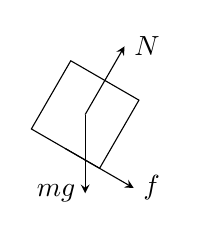
\begin{tikzpicture}
		\def\l{1};
		\def\b{1};
		\def\angle{30};
		\def\F{1};
	
		\begin{scope} [rotate around = {{-\angle}:({\l/2},{\b/2})}]
			\draw (0,0) rectangle (\l,\b);
			
			\coordinate (centre) at ({\l/2},{\b/2});
			\coordinate (base) at ({\l/2},0);
		\end{scope}
	
		\begin{scope}[-stealth]
			\draw (centre) -- ++(-90:\F) node [left] {$m g$};
			\draw (centre) -- ++({90 - \angle}:\F) node [right] {$N$};
			\draw (base) -- ++({-\angle}:\F) node [right] {$f$};
		\end{scope}
	\end{tikzpicture}
	\caption{Forces acting on the block in a rest frame if the block tends to move up the incline.}
\end{figure}

\begin{figure}[H]
	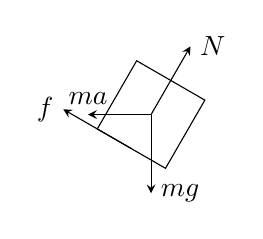
\begin{tikzpicture}
		\def\l{1};
		\def\b{1};
		\def\angle{30};
		\def\F{1};
			
		\begin{scope} [rotate around = {{-\angle}:({\l/2},{\b/2})}]
			\draw (0,0) rectangle (\l,\b);
			
			\coordinate (centre) at ({\l/2},{\b/2});
			\coordinate (base) at ({\l/2},0);
		\end{scope}
			
		\begin{scope}[-stealth]
			\draw (centre) -- ++(-90:\F) node [right] {$m g$};
			\draw (centre) -- ++({90 - \angle}:\F) node [right] {$N$};
			\draw (base) -- ++({180 - \angle}:\F) node [left] {$f$};
			\draw (centre) -- ++(180:0.8*\F) node [above] {$m a$};
		\end{scope}
	\end{tikzpicture}
	\caption{Forces acting on the block in the wedge frame if the block tends to move down the incline.}
\end{figure}

\begin{figure}[H]
	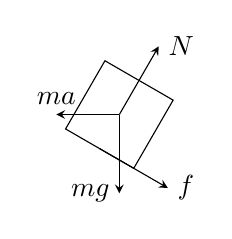
\begin{tikzpicture}
		\def\l{1};
		\def\b{1};
		\def\angle{30};
		\def\F{1};
			
		\begin{scope} [rotate around = {{-\angle}:({\l/2},{\b/2})}]
			\draw (0,0) rectangle (\l,\b);
			
			\coordinate (centre) at ({\l/2},{\b/2});
			\coordinate (base) at ({\l/2},0);
		\end{scope}
			
		\begin{scope}[-stealth]
			\draw (centre) -- ++(-90:\F) node [left] {$m g$};
			\draw (centre) -- ++({90 - \angle}:\F) node [right] {$N$};
			\draw (base) -- ++({-\angle}:\F) node [right] {$f$};
			\draw (centre) -- ++(180:0.8*\F) node [above] {$m a$};
		\end{scope}
	\end{tikzpicture}
	\caption{Forces acting on the block in the wedge frame if the block tends to move up the incline.}
\end{figure}
~\\
For the block to be stationary with respect to the wedge, the net forces on the block, in the frame of the reference of the wedge, are 0.\\
Therefore, if the block tends to move down the incline, at the threshold condition
\begin{align*}
	f_{\text{max}} \cos \theta + m a &= N \sin \theta\\
	f_{\text{max}} \sin \theta + N \cos \theta &= mg
\end{align*}
Therefore,
\begin{align*}
	\mu N \cos \theta + m a &= N \sin \theta\\
	\therefore N \sin \theta - \mu N \cos \theta &= m a\\
	\mu N \sin \theta + N \cos \theta &= mg\\
	\therefore \dfrac{\sin \theta - \mu \cos \theta}{\mu \sin \theta + \cos \theta} &= \dfrac{a}{g}\\
	\therefore a &= g \left( \dfrac{\sin \theta - \mu \cos \theta}{\mu \sin \theta + \cos \theta} \right)
\end{align*}\\
Therefore, if the block tends to move up the incline, at the threshold condition
\begin{align*}
	m a &= N \sin \theta + f_{\text{max}} \cos \theta\\
	N \cos \theta &= mg + f_{\text{max}} \sin \theta
\end{align*}
Therefore,
\begin{align*}
	m a &= N \sin \theta + \mu N \cos \theta\\
	N \cos \theta &= mg + \mu N \sin \theta\\
	\therefore m g &= N \cos \theta - \mu N \sin \theta\\
	\therefore \dfrac{a}{g} &= \dfrac{\sin \theta + \mu \cos \theta}{\cos \theta - \mu \sin \theta}\\
	\therefore a &= g \left( \dfrac{\sin \theta + \mu \cos \theta}{\cos \theta - \mu \sin \theta} \right)
\end{align*}
~\\
If the block tends to move down the incline,\\
If $\theta = 0$,
\begin{align*}
	a &= -\mu g\\
\end{align*}\\
If $\theta = \dfrac{\pi}{2}$, 
\begin{align*}
	a &= \dfrac{g}{\mu}\\
\end{align*}
~\\
If the block tends to move up the incline,\\
If $\theta = 0$, 
\begin{align*}
	a &= \mu g\\
\end{align*}\\
If $\theta = \dfrac{\pi}{2}$, 
\begin{align*}
	a &= -\dfrac{g}{\mu}\\
\end{align*}

\subsection*{Exercise 2}

\begin{tikzpicture}
	\def\R{2};
	\def\h{0.5};
	\def\angle{30};
	\def\F{1};
	
	\begin{scope}[-stealth, shift = {(\R,\R)}]
		\draw (0,0,0) -- (1,0,0) node [right] {$\hat{i}$};
		\draw (0,0,0) -- (0,1,0) node [above] {$\hat{j}$};
		\draw (0,0,0) -- (0,0,1) node [right] {$\hat{k}$};
	\end{scope}
	
	\draw (0,0) circle [radius = \R];
	
	\coordinate (mass) at ({180 + \angle}:{\R + \h});
	
	\fill (mass) circle [radius = 2pt];
	
	\draw [dashed] (0,0) -- (180:\R);
	\draw [dashed] (0,0) -- (mass);
	
	\node at ({180 + \angle/2}:1) {$\theta$};
	
	\draw [-stealth, thick] (mass) -- ++({90 + \angle}:\F) node [above left] {$v$};
	
	\draw [dashed] (0,{-(\R + 1)}) -- (0,{\R + 1});
	\node at (0,{\R + 0.5}) {\AxisRotator[rotate = 90]};
	\node [xshift = 10, yshift = 10] at (0,{\R + 0.5}) {$\omega$};
	
	\draw [stealth-, thick] (mass) -- ++(0:{(\R + \h)*cos(\angle)}) node [midway, below] {$r$};
\end{tikzpicture}

\begin{align*}
	\overrightarrow{F_{\text{centrifugal}}} &= - \overrightarrow{\omega} \times\left( \overrightarrow{\omega} \times \overrightarrow{r} \right)\\
	&= - m \omega^2 R_e \cos \theta \hat{i}
\end{align*}

\begin{align*}
	\overrightarrow{F_{\text{coriolis}}} &= -2 m \overrightarrow{\omega} \times \overrightarrow{v}\\
	&= -2 m \omega v \sin \theta \hat{k}
\end{align*}

\section*{Week 4 : Home Assignment}

\subsection*{Exercise 1}

\begin{figure}[H]
	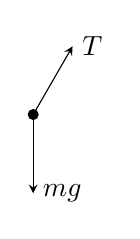
\begin{tikzpicture}
		\def\angle{30};
		\def\F{1};
		
		\fill (0,0) circle [radius = 2pt];
		
		\begin{scope}[-stealth]
			\draw (0,0) -- ({90 - \angle}:\F) node [right] {$T$};
			\draw (0,0) -- (-90:\F) node [right] {$mg$};
		\end{scope}
	\end{tikzpicture}
	\caption{Forces on the ball as seen from the rest frame.}
\end{figure}

\begin{figure}[H]
	\begin{tikzpicture}
		\def\angle{30};
		\def\F{1};
		
		\fill (0,0) circle [radius = 2pt];
		
		\begin{scope}[-stealth]
			\draw (0,0) -- ({90 - \angle}:\F) node [right] {$T$};
			\draw (0,0) -- (-90:\F) node [right] {$mg$};
			\draw (0,0) -- (180:\F) node [left] {$ma_0$};
		\end{scope}
	\end{tikzpicture}
	\caption{Forces on the ball as seen from the train frame of reference.}
\end{figure}
~\\
In the frame of reference of the train,
\begin{align*}
	m g &= T \cos \theta\\
	m a_0 &= T \sin \alpha\\
	\therefore \dfrac{a_0}{g} &= \tan \theta\\
	\therefore \theta &= \tan^{-1} \dfrac{a_0}{g}
\end{align*}\\
~\\
Let the position of the ball at $t = T$ be 0.\\
In the frame of reference of the train,
\begin{align*}
	\overrightarrow{a'} &= - a_0 \hat{i} - g \hat{j}\\
	\intertext{As $v'(t = T) = 0$,}
	\therefore \overrightarrow{v'} &= - a_0 (t - T) \hat{i} - g (t - T) \hat{j}\\
	\intertext{As $r'(t = T) = 0$,}\\
	\therefore \overrightarrow{r'} &= - \dfrac{1}{2} a_0 (t - T)^2 \hat{i} - \dfrac{1}{2} g (t - T)^2 \hat{j}
\end{align*}
In the rest frame,
\begin{align*}
	\overrightarrow{a} &= - g \hat{j}\\
	\overrightarrow{v}(t = 0) &= a_0 T \hat{i}\\
	\therefore \overrightarrow{r} &= a_0 T (t - T) \hat{i} - \dfrac{1}{2} g (t - T)^2
\end{align*}

\subsection*{Exercise 2}

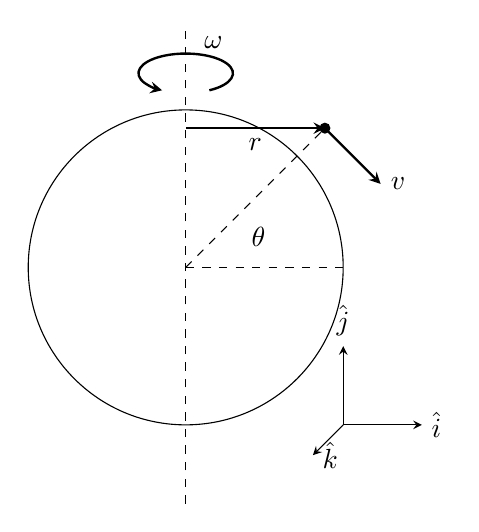
\begin{tikzpicture}
	\def\R{2};
	\def\h{0.5};
	\def\angle{45};
	\def\F{1};
	
	\begin{scope}[-stealth, shift = {(\R,-\R)}]
		\draw (0,0,0) -- (1,0,0) node [right] {$\hat{i}$};
		\draw (0,0,0) -- (0,1,0) node [above] {$\hat{j}$};
		\draw (0,0,0) -- (0,0,1) node [right] {$\hat{k}$};
	\end{scope}
	
	\draw (0,0) circle [radius = \R];
	
	\coordinate (mass) at ({\angle}:{\R + \h});
	
	\fill (mass) circle [radius = 2pt];
	
	\draw [dashed] (0,0) -- (0:\R);
	\draw [dashed] (0,0) -- (mass);
	
	\node at ({\angle/2}:1) {$\theta$};
	
	\draw [-stealth, thick] (mass) -- ++({-90 + \angle}:\F) node [right] {$v$};
	
	\draw [dashed] (0,{-(\R + 1)}) -- (0,{\R + 1});
	\node at (0,{\R + 0.5}) {\AxisRotator[rotate = 90]};
	\node [xshift = 10, yshift = 10] at (0,{\R + 0.5}) {$\omega$};
	
	\draw [stealth-, thick] (mass) -- ++(180:{(\R + \h)*cos(\angle)}) node [midway, below] {$r$};
\end{tikzpicture}\\

\begin{align*}
	m &= 2 \si{\kilogram}\\
	v &= 500 \si{\metre\per\second}\\
	\theta &= 45 \si{\degree}\\
	R_e &= 6.37 \times 10^6 \si{\metre}
\end{align*}

\begin{align*}
	\overrightarrow{F_{\text{centrifugal}}} &= - m \overrightarrow{\omega} \times \left( \overrightarrow{\omega} \times \overrightarrow{r} \right)\\
	&= m \omega^2 R_e \cos \theta \hat{i}\\
	&= m \left( \dfrac{2 \pi}{T} \right)^2 R_e \cos \theta \hat{i}\\
	&= m \dfrac{4 \pi^2}{T^2} R_e \cos \theta \hat{i}\\
	&= (2) \dfrac{4 \pi^2}{(86400)^2} (6.37 \times 10^6) \dfrac{1}{\sqrt{2}} \hat{i}\\
	&= \dfrac{8 \pi^2}{746496} (6.37 \times 10^2) \dfrac{1}{\sqrt{2}} \hat{i}\\
	&= \dfrac{(8)(6.37)}{(746496)(\sqrt{2})} \times 10^2 \hat{i}\\
	&= \dfrac{5096}{1055704.7675} \hat{i}\\
	&= 0.00482710712 \hat{i} \si{\newton}\\
	&= 4.82710712 \times 10^{-3} \hat{i} \si{\newton}\\
	\therefore F_{\text{centrifugal}} &= 4.82710712 \times 10^{-3} \si{\newton}
\end{align*}

\begin{align*}
	\overrightarrow{F_{\text{coriolis}}} &= - 2 m \overrightarrow{\omega} \times \overrightarrow{v}\\
	&= 2 m \omega v \dfrac{1}{\sqrt{2}} \hat{k}\\
	&= (2) (2) \dfrac{2 \pi}{86400} (500) \dfrac{1}{\sqrt{2}} \hat{k}\\
	&= \dfrac{40}{864} \cdot \dfrac{1}{\sqrt{2}} \hat{k}\\
	&= \dfrac{5 \sqrt{2}}{216} \pi \hat{k}\\
	&= 0.102845 \hat{k} \si{\newton}\\
	\therefore F_{\text{coriolis}} &= 1.02845 \times 10^{-1} \si{\newton}
\end{align*}

\begin{align*}
	F_{\text{gravity}} &= m g\\
	&= (2) (9.81)\\
	&= 19.62 \si{\newton}
\end{align*}
Therefore, the Coriolis and centrifugal forces are very small compared to gravity.

\subsection*{Exercise 5}

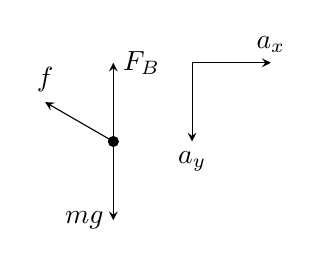
\begin{tikzpicture}
	\def\angle{30};
	\def\F{1};

	\coordinate (mass) at (0,0);
	
	\fill (mass) circle [radius = 2pt];
	
	\begin{scope}[-stealth]
		\draw (mass) -- ++({180 - \angle}:\F) node [above] {$f$};
		\draw (mass) -- ++(-90:\F) node [left] {$mg$};
		\draw (mass) -- ++(90:\F) node [right] {$F_B$};
		\draw ($ (mass) + (1,1) $) -- ++(-90:\F) node [below] {$a_y$};
		\draw ($ (mass) + (1,1) $) -- ++(0:\F) node [above] {$a_x$};
	\end{scope}
\end{tikzpicture}\\

\begin{align*}
	m a_y &= - F_B + m g - f \sin \theta\\
	&= - \rho_W V g + m g - k v_x\\
	&= - \dfrac{4}{3} \pi \rho_W R^3 g + m g - k v_y\\
	m a_x &= - f \cos \theta\\
	&= - k v_x
\end{align*}
Therefore,
\begin{align*}
	m \ddot{x} &= - k \dot{x}\\
	m \ddot{y} &= - k \dot{y} - \dfrac{4}{3} \pi \rho_W R^3 g + m g
\end{align*}
Therefore,
\begin{align*}
	\dod{v_x}{t} &= - \dfrac{k}{m} v_x\\
	\therefore \dfrac{\dif v_x}{v_x} &= - \dfrac{k}{m} \dif t\\
	\therefore \ln v_x  - \ln v_0 \cos \theta &= - \dfrac{k}{m} t \\
	\therefore \dfrac{v_x}{v_0 \cos \theta} &= e^{-\sfrac{kt}{m}}\\
	\therefore v_x &= v_0 \cos \theta e^{-\sfrac{kt}{m}}
\end{align*}
~\\
\begin{align*}
	\dod{v_y}{t} &= - \dfrac{k}{m} v_y - \dfrac{\rho_W V g}{\rho_B g} + g\\
	&= g \left( 1 - \dfrac{\rho_W}{\rho_B} \right) - \dfrac{k}{m} v_y
\end{align*}
Let 
\begin{align*}
	u &= g \left( 1 - \dfrac{\rho_W}{\rho_B} \right) - \dfrac{k}{m} v_y\\
	\therefore \dif u &= - \dfrac{k}{m} \dif v_y
\end{align*}
Let
\begin{align*}
	A &= g \left( 1 - \dfrac{\rho_W}{\rho_B} \right)\\
	B &= \dfrac{k}{m}
\end{align*}
Therefore,
\begin{align*}
	\therefore \dfrac{\dif u}{u} &= - \dfrac{k}{m} v_y \dif t\\
	\therefore \ln u &= - \dfrac{k}{m} v_y t + c\\
	\therefore v_y &= \dfrac{A}{B} t + \left( v_0 \sin \theta - \dfrac{A}{B} \right)e^{-Bt}
\end{align*}
At $t = t_0$, $v_y(t) = 0$.
\begin{align*}
	t_0 &= \dfrac{1}{B} \ln \left( \dfrac{v_y \sin \theta + \sfrac{A}{B}}{\sfrac{A}{B}} \right)\\
	\therefore y_{\textnormal{max}} &= \dfrac{v_0 \sin \theta}{B} - \dfrac{A}{B^2} \ln \left( \dfrac{B v_0 \sin \theta}{A} + 1 \right)
\end{align*}

\end{document}